\providecommand{\main}{../../../..}
\documentclass[\main/dresen_thesis.tex]{subfiles}

\begin{document}
  \label{sec:monolayers:methods:superballFF}
    \begin{figure}[tb]
      \centering
      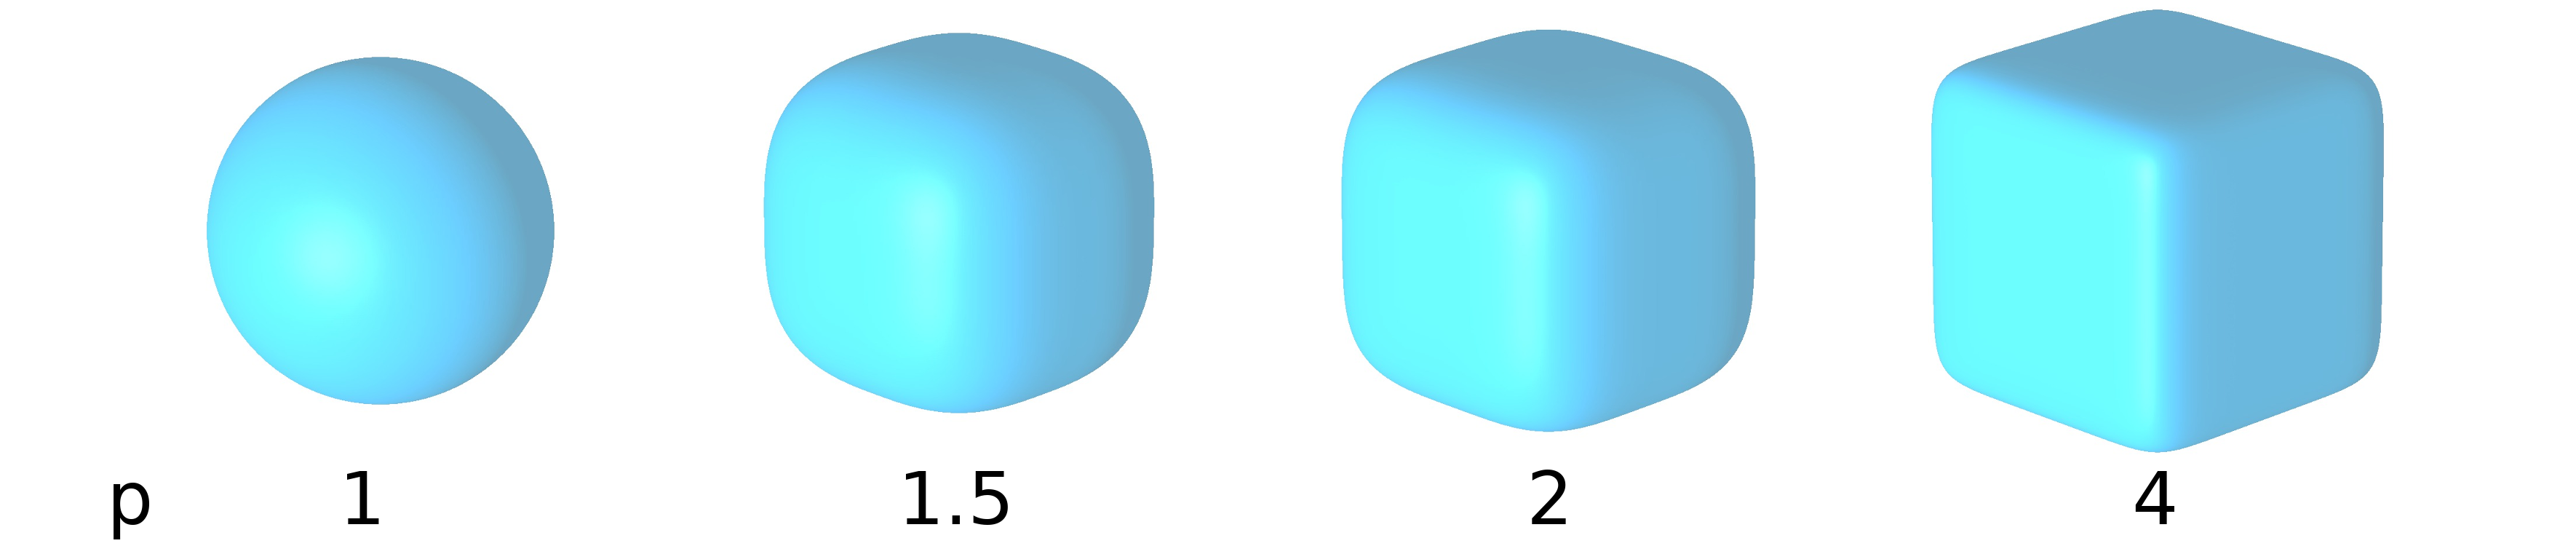
\includegraphics{appendix_superballShapes}
      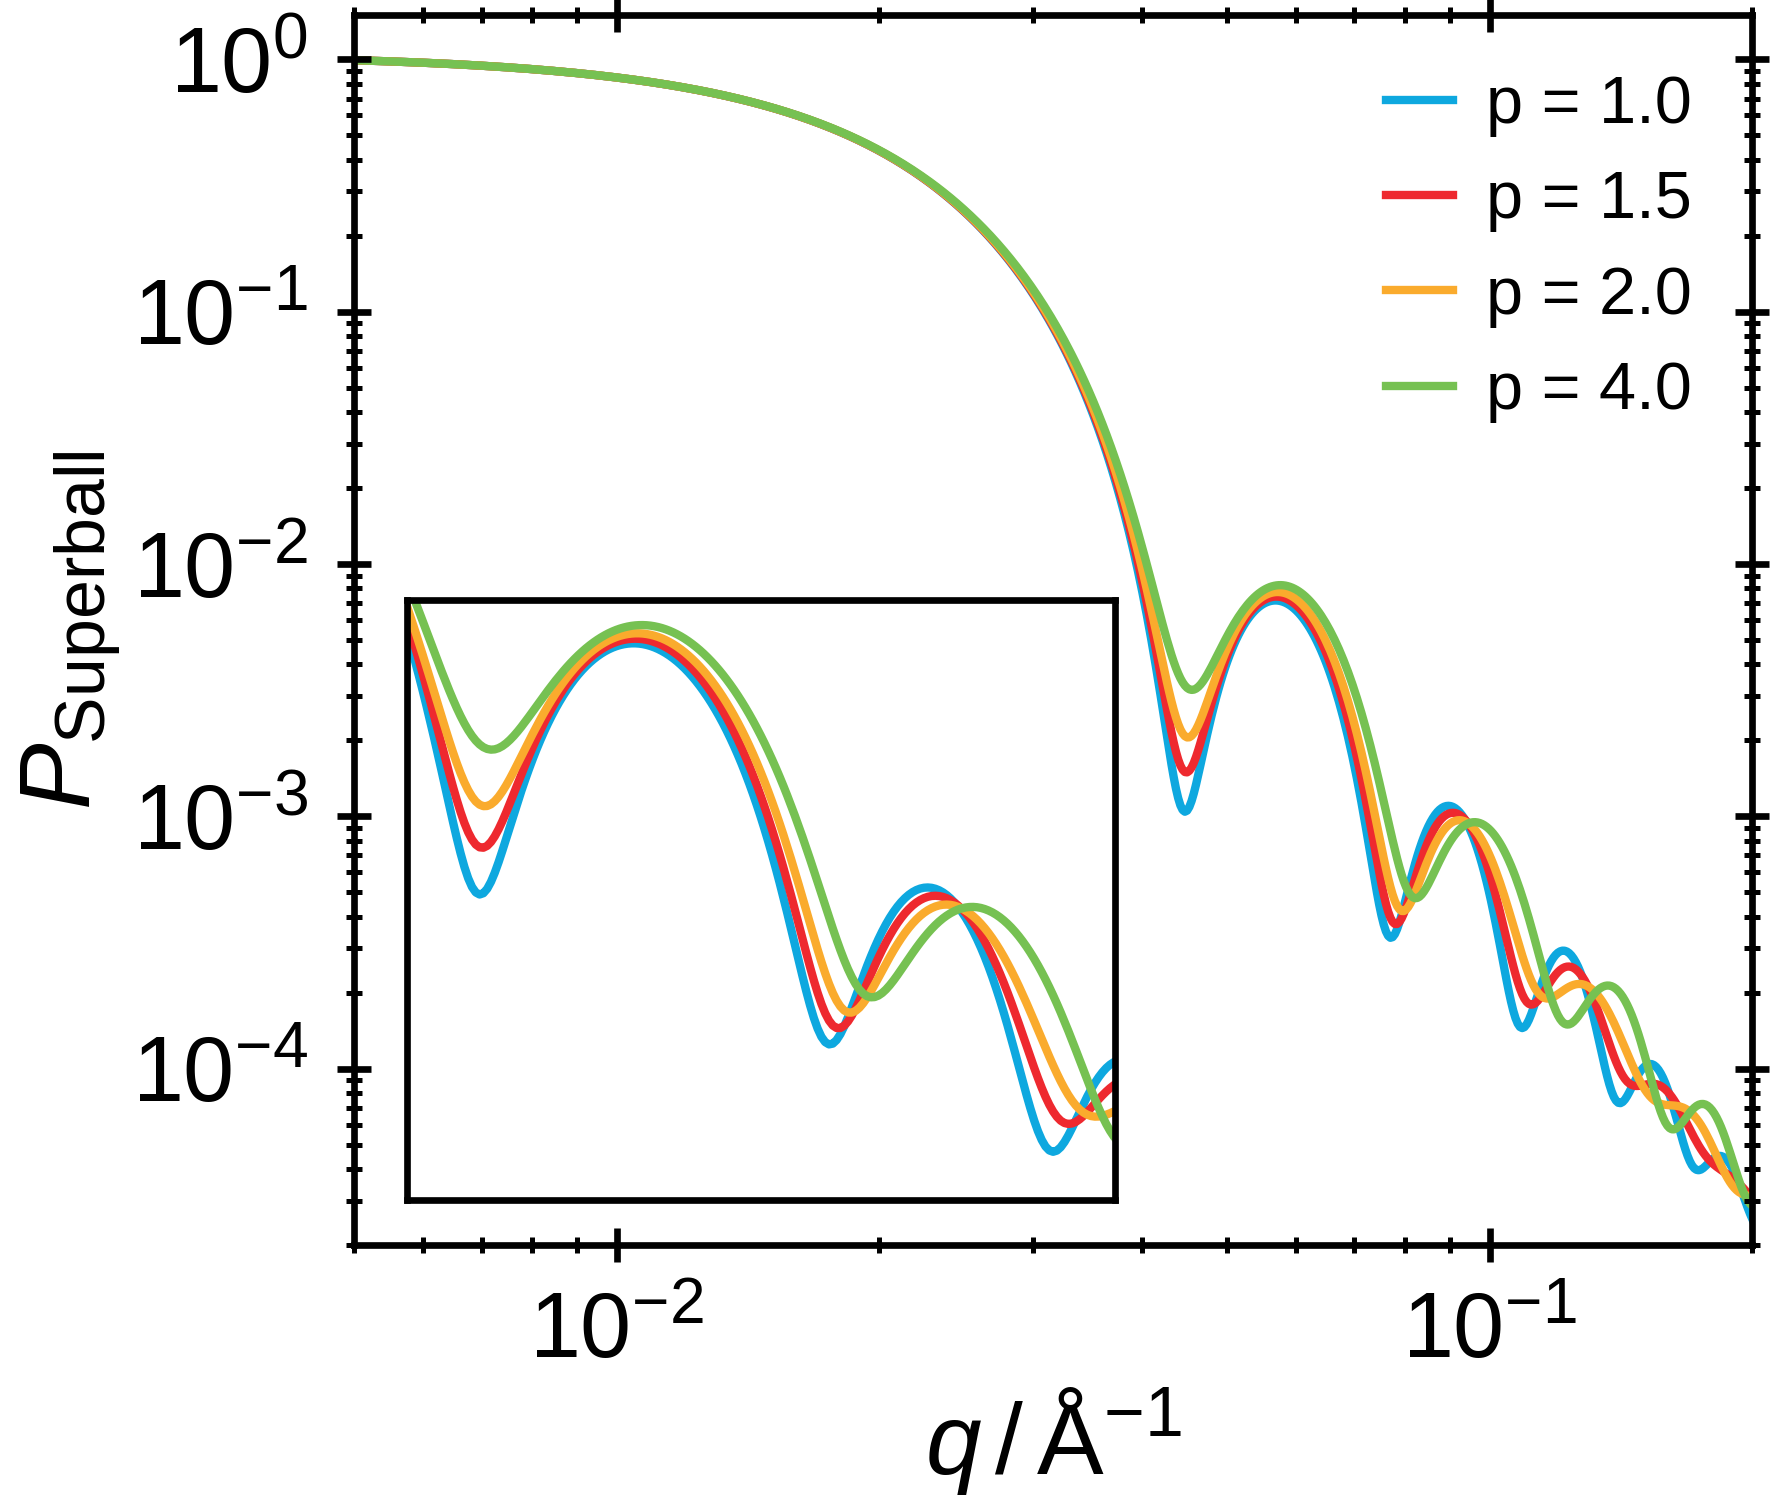
\includegraphics{monolayers_SAS_SuperballFF}
      \caption{\label{fig:monolayers:nanoparticle:superballShapes}Visualization of the superball shape for varied $p$ (left) and the corresponding form factor simulated for a size distribution of $\sigma_R \eq 5 \%$ (right).}
    \end{figure}
    To evaluate the small-angle scattering data quantitatively, the experimental data is used to fit the parameters of a superball form factor that was derived and implemented in the course of this thesis.
    A superball is a mathematical shape that can be used to describe rounded cubes and it's volume is defined by
    \begin{align}
      x^{2p} + y^{2p} + z^{2p} < R^{2p},
    \end{align}
    where $R$ is the radius of the superball and $p$ describes whether the body is closer to a sphere or a cube.
    \reffig{fig:monolayers:nanoparticle:superballShapes} shows the surface of a superball for varied $p$.
    For $p\eq 1$ the superball is equivalent to the definition of a sphere and for $p \rightarrow \infty$ the superball converges to a cube with edge length $a \eq 2R$.

    The full description and derivation of the superball properties and formfactor is described in \refapp{ch:appendix:numericalMethods:superballFormfactor}.
    The form factor amplitude of an oriented superball is given by the integral
    \begin{align}
      \begin{split}
        p_\mathrm{orient}(\vec{q}) &\eq \frac{2R^3}{q_z R V_p} \int_{-1}^{1} \dint x \int_{-\gamma}^{\gamma} \dint y \cos(R q_x x + R q_y y)  \sin (q_z R \zeta),\\
        &\mathrm{with}\\
        \gamma \eq& \sqrt[2p]{1-x^{2p}}, \\
        \zeta \eq& \sqrt[2p]{1-x^{2p} -y^{2p}}.
      \end{split}
    \end{align}

    For the data fit, an average over the size distribution $\Lambda(R)$ and an orientation average over one octant with solid angle $\tfrac{\pi}{2}$ is performed as described in \refapp{ch:appendix:numericalMethods:superballFormfactor}, and the form factor is multiplied with a parameter for the particle density and contrast to the solvent
    \begin{align}
      \label{eq:superballFormfactorIntensity}
      I_\mathrm{Superball}(q) = \frac{2 I_0 \Delta \rho^2}{\pi} \int_0^{\pi/2} \dint \varphi \int_0^{\pi/2} \dint \theta \sin (\theta)  \int_0^\infty \dint R \Lambda(R) V_p^2 |p_\mathrm{orient.}(\vec{q}; R)|^2,
    \end{align}

    To account for an oleic acid surfactant of the nanoparticles, the superball is assumed to have a core-shell structure.
    This is done by replacing the amplitude in \refeq{eq:superballFormfactorIntensity} by
    \begin{align}
      \begin{split}
        &\Delta \rho V_p p_\mathrm{orient.}(\vec{q}; R) \rightarrow\\
        &\hspace{1cm}(\rho_\mathrm{shell} - \rho_\mathrm{solvent}) V_p^{R+D} p_\mathrm{orient.}(\vec{q}; R+D) + (\rho_\mathrm{core} - \rho_\mathrm{shell}) V_p^{R} p_\mathrm{orient.}(\vec{q}; R),
      \end{split}
    \end{align}
    where $D$ is the thickness of the shell, $V_p^{R+D}$ the total particle volume and $V_p^{R}$ the core volume.

    The superball allows to transition continuously from a sphere to a cube by a single parameter $p$.
    The form factor in the right plot of \reffig{fig:monolayers:nanoparticle:superballShapes}, simulated for a typical minimal size distribution of $\sigma_R \eq 5 \%$, shows that during this transition the first form factor minima decreases in sharpness, whereas the second order form factor maxima shifts to larger scattering vector magnitudes.
    Thus if experimental data for particles with a small size distribution is given, the parameter $p$ can additionally be refined.
\end{document}